\section{SMT Model}

Similarly to the SAT model, the SMT model is structured based on its two tasks: \textbf{Satisfiability} and \textbf{Optimization}.
We encode both the satisfiability and optimization phases in QF\_LIA (Quantifier-Free Linear Integer Arithmetic) because it lets us combine Boolean decisions with integer sums and comparisons directly, avoiding complex encodings of counters in pure SAT.

\subsection{Decision Variables}

\subsubsection{Satisfiability}

The decision variables for this task are:
\begin{itemize}
    \item $match\_schedule_{p,w,m} \in \{\text{true}, \text{false}\}$: true if, and only if, the match $m \in M$ is scheduled for period $p \in P$ of week $w \in W$.
    \item $home_{p,w} = t \in T$: if t is the home team in the match in period $p \in P$ of week $w \in W$.
    \item $away_{p,w} = t \in T$: if t is the away team in the match in period $p \in P$ of week $w \in W$.
\end{itemize}

\subsubsection{Optimization}
To optimize the balance of the number of games played at home and away for each team, the following variables are utilized:
\begin{itemize}
    \item $flip\_slot_{p,w} \in \{\text{true}, \text{false}\}$: % similarly to other models, it defines which team plays at home and which away in the matchup $(t_1, t_2)$ in week w and period p. 
    if the value is false, $rb_{p, w, 0}=t_1$ plays at home; otherwise it is true, then $rb_{p, w, 1}=t_2$ is the one playing at home.
    
    \item $home\_eff_{p,w},\, away\_eff_{p,w} \in T$: are, respectively, the effective home and effective away teams after the slot flip decisions.
\end{itemize}

\subsection{Objective Function}

The optimization goal is to minimize the maximum imbalance $k$ between the number of home and away games played by each team, respectively $H_t$ and $A_t$, throughout the tournament. Formally,

\[
k^* = \underset{k \in \mathbb{N}}{\text{argmin}} \left( \forall t \in T. |H_t - A_t| \leq k \right)
\]

where:
\[
H_t = \sum_{p,w} \mathbbm{1}[\,home\_eff_{p,w} = t\,], 
\quad
A_t = \sum_{p,w} \mathbbm{1}[\,away\_eff_{p,w} = t\,].
\]
The effective home and away variables are computed by considering slot flips:

\begin{align*}
home\_eff_{p,w} =& \text{ite}(flip\_slot_{p,w},\, away_{p,w},\, home_{p,w}), \\
away\_eff_{p,w} =& \text{ite}(flip\_slot_{p,w},\, home_{p,w},\, away_{p,w}).
\end{align*}
where ite stands for "if then else" statement.

\subsection{Constraints}

\subsubsection{Each match is assigned to a unique period each week}

Each period in each week is assigned to exactly one match:

\[
\forall p \in P,\, w \in W: 
\sum_{m \in M} match\_schedule_{p,w,m} = 1.
\]
Each match is assigned to exactly one period each week:

\[
\forall m \in M,\, w \in W: 
\sum_{p \in P} match\_schedule_{p,w,m} = 1.
\]

\subsubsection{Binding team assignments}
The teams playing in $match\_schedule_{p, w, m}$ are linked to the corresponding variables $home_{p, w}$ and $away_{p, w}$ based on the values of $rb_{m, w}$ as follows:

$$
\forall p \in P,\, w \in W.(match\_schedule_{p,w,m} \leftrightarrow (home_{p,w} = rb_{m,w,0} \ \wedge \ away_{p,w} = rb_{m,w,1})
\big)
$$

\subsubsection{Every team plays at most twice in the same period}

For each team $t$ and each period $p$, we count how many times $t$ appears either as home or away in that period over all weeks and constraint the count to not exceed 2:

\[
\forall t \in T,\, p \in P: 
\sum_{w \in W} \sum_{m \in M} 
\big(
[\,rb_{m,w,0} = t \lor rb_{m,w,1} = t\,] \cdot [\,match\_schedule_{p,w,m}\,]
\big) \leq 2.
\]

\subsubsection{Symmetry breaking}

To reduce equivalent permutations of the solutions, the first match is fixed:

\[
match\_schedule_{0,0,0} = \text{true}.
\]

\subsection{Validation}

\subsubsection{Experimental Design}

Solver performance is measured in two stages:
\begin{enumerate}
  \item \textbf{Satisfiability}: Produce a single \texttt{.smt2} file that encodes match assignments, period-limit, and symmetry breaking constraints as linear arithmetic formulas. The solver then finds an initial feasible schedule.
  \item \textbf{Optimization}: Perform a binary search over 
  \[
    k \in \{1,2,\dots,N/2\}.
  \]
  For each candidate \(k\), generate a new \texttt{.smt2} file that
  \begin{itemize}
    \item has the base \(home/away\) assignments,
    \item adds boolean \texttt{flip\_slot} variables,
    \item defines effective \(home\_eff,away\_eff\) via \texttt{ite},
    \item asserts \(\lvert H_t - A_t\rvert \le k\) using integer counters \(H_t,A_t\).
  \end{itemize}
  This produces \(\log_2(N) - 1\) optimization files.
\end{enumerate}

The total runtime is measured from the start of the satisfiability phase until either a solution for \(k = 1\) is found or the 300\,s timeout is reached.
We tested the following solvers: Z3 4.15.1.0 and CVC5 1.3.0 and present our findings in table \ref{table:smt-result}. 

\subsubsection{Experimental results}

The experimental results show that Z3 performs significantly better than CVC5 in terms of solving time and scalability. Specifically, Z3 solved instances up to $N=22$, while CVC5 handled only smaller instances up to $N=8$.

\begin{table}[H]
\centering
\small
\begin{tabular}{|c|c|c|}
\toprule
\textbf{N} & \textbf{Z3} & \textbf{CVC5} \\
\midrule
6  & \textbf{1}   & \textbf{1}   \\
8  & \textbf{1}   & \textbf{1}   \\
10 & \textbf{1}   & N/A \\
12 & \textbf{1}   & N/A \\
14 & \textbf{1}   & N/A \\
16 & \textbf{1}   & N/A \\
18 & \textbf{1}   & N/A \\
20 & \textbf{1}  & N/A \\
22 & \textbf{1} & N/A \\
24 & N/A & N/A \\
\bottomrule
\end{tabular}
\caption{SMT optimization solver results}
\label{table:smt-result}
\end{table}

% \begin{figure}[H]
% \centering
% 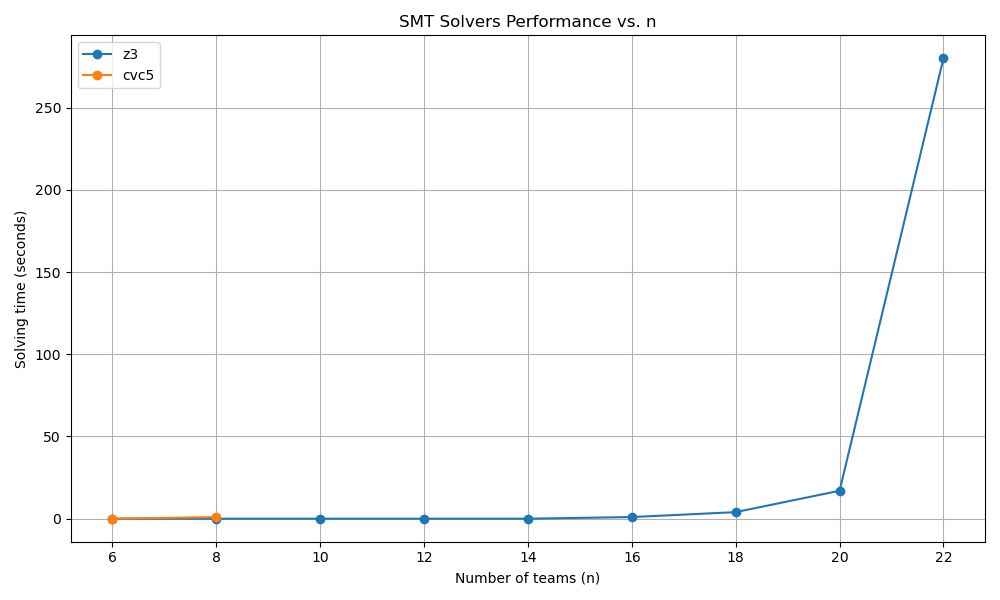
\includegraphics[width=0.8\linewidth]{img/SMT-result.png}
% \caption{SMT solution example}
% \label{fig:smt-result}
% \end{figure}
